\chapter{Lecture 7}

%--- 信息 ----
\begin{center}
    讲师:王立威 \qquad
    课程时间:25.Apr.1st \qquad 
    笔记:25.June.8th
\end{center}

\bigskip

接着上一课程未解决的问题,我们如何定义一个确定对象的“最短描述长度”。此前,我们已经将这个对象的范围缩小到$x \in \{0,1\}^*$,加上Turing给出的计算模型,我们已经具备定义Kolmogorov复杂度的能力了!(关于下面用到的通用Turing机(universal Turing machine)这一概念,请自行浏览资料)
\begin{definition}[Kolmogorov复杂度]
    对于一个字符串$x \in \{0,1\}^*$,其对于一个通用Turing机$U$的\textbf{Kolmogorov复杂度}(complexity)定义为 
\[
K_U(x) := \min_{p, U(p)=x} \abs{p}
\]

也就是$U$要决定$x$所需的最短“代码”长度,这也简称为K-复杂度,并简写为$K(x)$.
\end{definition}

若没有学过Turing机相关的知识,可以暂时理解成$U$是某个固定的编程语言,例如C++或Python等。以下命题说明了上面将$U$简写是合理的:
\begin{proposition}
    设$U, U'$是两个通用Turing机,那么存在一个常数$c \in \N$使得对于任意$x \in \{0, 1\}^*$,如下不等式成立 
    \[
    K_U(x) \le K_{U'}(x) + c
    \]

    其中$c$只依赖于$U,U'$而不依赖于$x$.
\end{proposition}

但这个定义听起来很难实践。一种尝试计算$x$的K-复杂度的方式,是从根据长度小到大遍历所有的$p$(由于$K_U(x)$一定存在有界,所以需要遍历的$p$是有限多的),但这会遇到一个难题:“停机问题”。我们无法判断对于特定的$p$,$U$是否会停机。 归根结底,这是因为$K_U$本质上是不可以计算的!
\begin{theorem}
    $K_U(x)$是不可计算的. 
\end{theorem}
\begin{proof}
    这里只给出大致的思想,UTM的细节略去。假设存在一个算法$P_0$,可以对于任意$x$计算$K_U(x)$. 

    记$\abs{P_0} = l$,下面给出一个新的算法$P_0'$。首先我们将$\{0,1\}^*$中的元素排序成$s_1,s_2,\dots,s_i,\dots$。
    
    $P_0'$如下:
    \begin{itemize}
        \item 令变量$i$遍历$1,2,\dots$
        \begin{itemize}
            \item 使用$P_0$计算$K_U(s_i)$
            \item 若$K_U(s_i) \ge L$,则输出$s_i$
        \end{itemize}
    \end{itemize}

    那么可见$\abs{P_0'} = l + \al \log L + \be$($\al, \be$常数). 而$P_0'$可以决定识别字符串$s$,其中$K_U(s) \ge L$。但根据K-复杂度的定义,会有 
    \[
    L \le K_U(s) \le \abs{P_0'} = l + \al \log L + \be
    \]

    所以取$L$充分大便可得到矛盾. 因此$K_U$不可计算.
\end{proof}

关于这部分告一段落,我们来看概率分布估计的问题,也就是说对于一些函数$g_i$,已知$\E_X\sim P [g_i(X)]$的值,求原始分布$P$。 这类问题往往具有无穷多个解,我们应当关心其中某个具有优良性质的。 
    \begin{definition}[最大熵估计]
        给定一族函数$\{g_i(x)\}_{i\in I}$和$\{r_i\}_{i \in I}$。\textbf{最大熵估计}指的是如下问题的解 
        
        \begin{align*}
            \maximize_{f} \ & -\int f(x) \ln f(x) \dx \\
            \text{s.t.} \ & \int f(x) \dx = 1 \\
            \ & \int g_i(x)f(x) \dx = r_i\quad ,i\in I
        \end{align*}
    \end{definition}

这里将所谓“熵”从$\log_2$替换成$\ln$是因为他们只差一个倍数。 我们试着求解一个最大熵问题:
\begin{example}
    给定一个连续型随机变量$X$及其p.d.f. $f(x)$,已知
    \[
    \E[X] = 0, \qquad \var(X) = \sigma^2
    \]
    
    求最大熵分布. 
\end{example}
\begin{solution}
    一般而言,这类问题的通法时使用Lagrange乘子和变分。不过这里我们可以给出一个使用K-L散度的解法。 


\end{solution}
% \begin{figure}[H]
%     \centering
%     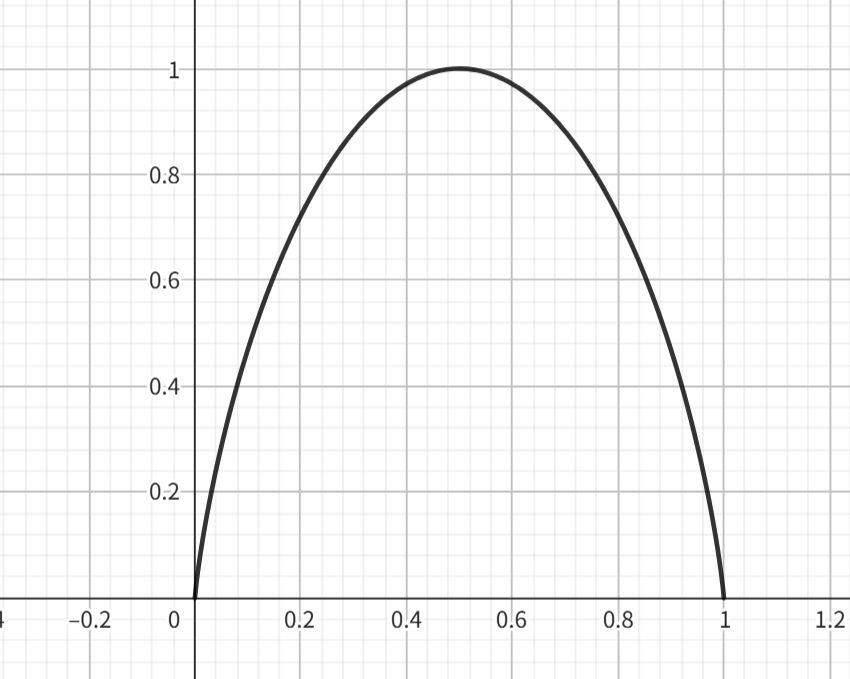
\includegraphics[width=.6\textwidth]{images/c2_1.png}
%     \caption{$H=x\log 1/x + (1-x)\log 1/(1-x)$的图像}
% \end{figure}